\documentclass{article}

\usepackage{tikz}
\usetikzlibrary{turtle}
\begin{document}

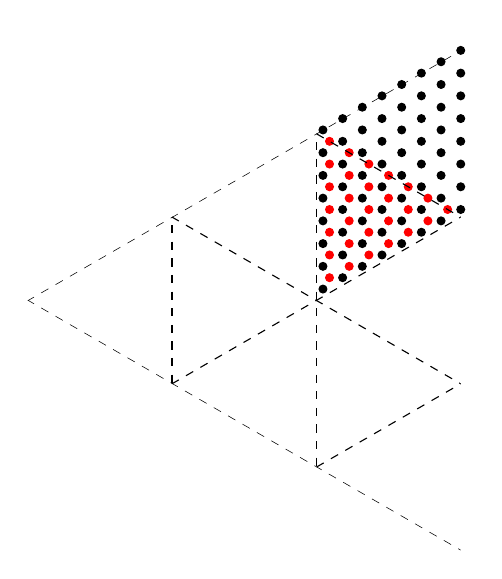
\begin{tikzpicture}[scale=.5, turtle/distance=8/3*1.732]

%\clip (-9,-9)--(-9,9)--(9,9)--(9,-9)--cycle;

%\clip (-7.3,0)--(4.15, 3.81666*1.7320508)--(4.15, -3.81666*1.7320508)--cycle;
%\clip (-7,0)--(4, 3.66666*1.7320508)--(4, -3.66666*1.7320508)--cycle;

%\clip (-3.5, -4*1.7320508/2)--(-3.5, 4*1.7320508/2)--(2.5,
%4*1.7320508/2)--(2.5, -4*1.7320508/2)--cycle;

%\fill[gray!50, xshift=-.3333cm] (-7,0)--(4, 11/3*1.7320508)--(4, -11/3*1.7320508)--cycle;
%\draw[dashed, xshift=-.3333cm] (-7,0)--(4, 11/3*1.7320508)--(4, -11/3*1.7320508)--cycle;

\begin{scope}[rotate=-120]
\clip [turtle={home, lt=60, fd, lt=60, fd, lt=120, fd, lt=60, fd}];
\begin{scope}[xshift=-.33333cm]
\foreach \x in {-14,-13,...,14}{% Two indices running over each
    \foreach \y in {-10,-9,...,10}{% node on the grid we have drawn
        \node[draw,circle,inner sep=1pt,fill] at (\x-\y/2,1.7320508*\y/2) {};}}
\end{scope}
\end{scope}

\begin{scope}[rotate=120]
\clip [rotate=120, turtle={home, lt=60, fd, lt=60, fd, lt=120, fd, lt=60, fd}];
\begin{scope}[xshift=-.33333cm]
\foreach \x in {-14,-13,...,14}{% Two indices running over each
    \foreach \y in {-10,-9,...,10}{% node on the grid we have drawn
        \node[draw,circle,inner sep=1pt,fill] at (\x-\y/2,1.7320508*\y/2) {};}}
\end{scope}
\end{scope}

\begin{scope}
\clip [rotate=-120, turtle={home, lt=60, fd, lt=60, fd, lt=120, fd, lt=60, fd}];
\begin{scope}[xshift=-.33333cm]
\foreach \x in {-14,-13,...,14}{% Two indices running over each
    \foreach \y in {-10,-9,...,10}{% node on the grid we have drawn
        \node[draw,circle,inner sep=1pt,fill] at (\x-\y/2,1.7320508*\y/2) {};}}
\end{scope}
\end{scope}

\begin{scope}[xscale=-1]
\begin{scope}[rotate=-120]
\clip [rotate=60, turtle={home, lt=60, fd, lt=120, fd, lt=120, fd}];
\begin{scope}[xshift=-.33333cm]
\foreach \x in {-14,-13,...,14}{% Two indices running over each
    \foreach \y in {-10,-9,...,10}{% node on the grid we have drawn
        \node[draw,red, circle,inner sep=1pt,fill] at (\x-\y/2,1.7320508*\y/2) {};}}
\end{scope}
\end{scope}
\end{scope}

\begin{scope}[xscale=-1]
\begin{scope}[rotate=120]
\clip [rotate=180, turtle={home, lt=60, fd, lt=120, fd, lt=120, fd}];
\begin{scope}[xshift=-.33333cm]
\foreach \x in {-14,-13,...,14}{% Two indices running over each
    \foreach \y in {-10,-9,...,10}{% node on the grid we have drawn
        \node[draw,red, circle,inner sep=1pt,fill] at (\x-\y/2,1.7320508*\y/2) {};}}
\end{scope}
\end{scope}
\end{scope}

\begin{scope}[xscale=-1]
\clip [rotate=300, turtle={home, lt=60, fd, lt=120, fd, lt=120, fd}];
\begin{scope}[xshift=-.33333cm]
\foreach \x in {-14,-13,...,14}{% Two indices running over each
    \foreach \y in {-10,-9,...,10}{% node on the grid we have drawn
        \node[draw,red, circle,inner sep=1pt,fill] at (\x-\y/2,1.7320508*\y/2) {};}}
\end{scope}
\end{scope}



\begin{scope}
\clip[xshift=-.33333cm] (-7,0)--(4, 11/3*1.7320508)--(4,-11/3*1.7320508)--cycle;

\draw[dashed] (0, 10*1.7320508/2)--(0, -5*1.7320508);
\draw[dashed] (-11/3, 10*1.7320508/2)--(-11/3, -5*1.7320508);

\draw[dashed] (11/3, 10*1.7320508/2)--(11/3, -5*1.7320508);
\draw[dashed] (-15-7-1/3, 5*1.7320508)--(15-7-1/3, -5*1.7320508);
\draw[dashed] (-15, 5*1.7320508)--(15, -5*1.7320508);
\draw[dashed] (-15+7+1/3, 5*1.7320508)--(15+7+1/3, -5*1.7320508);

\draw[dashed] (-15-7-1/3, -5*1.7320508)--(15-7-1/3, 5*1.7320508);
\draw[dashed] (-15, -5*1.7320508)--(15, 5*1.7320508);
\draw[dashed] (-15+7+1/3, -5*1.7320508)--(15+7+1/3, 5*1.7320508);

\end{scope}


\end{tikzpicture}

\end{document}
